\chapter{Réalisation de l'application}



\section{les outils de développement}

\subsection{Java Enterprise Edition }

\begin{figure}[H]
    \centering
    \fbox{
\includegraphics[width=50mm,scale=0.5]{technologie/java.png}}
    \caption{Logo Java EE}
\end{figure}
La plateforme Java Entreprise (Java EE) est un ensemble de spécifications coordonnées et pratiques qui permettent des solutions pour le développement, le déploiement, et de la gestion des applications multi-tiers centralisées sur un serveur. Construite sur la plateforme de Java 2 édition standard (Java SE), la plateforme Java EE ajoute les possibilités nécessaires pour fournir une plateforme complète, stable, sécurisée, et rapide de Java au niveau entreprise. 
La plateforme Entreprise fournit un ensemble de services permettant aux composants de dialoguer entre eux.
\subsection{Eclipse Integrated Development Environment}
\begin{figure}[H]
    \centering
    \fbox{
\includegraphics[width=50mm,scale=0.5]{technologie/eclipse.png}}
    \caption{Logo Eclipse IDE}
\end{figure}
Eclipse IDE est un environnement de développement intégré libre extensible, universel et polyvalent, permettant potentiellement de créer des projets de développement (application web dans notre cas) mettant en œuvre le langage Java.

La spécificité d'Eclipse IDE vient du fait de son architecture totalement développée autour de la notion de plug-in : toutes les fonctionnalités de cet atelier logiciel sont développées en tant que plug-in.

\subsection{Serveur Tomcat}
\begin{figure}[H]
    \centering
    \fbox{
\includegraphics[width=50mm,scale=0.5]{technologie/tomcat.png}}
    \caption{Logo Tomcat Server }
\end{figure}
Apache Tomcat est un conteneur web libre de servlets et JSP Java EE. Issu du projet Jakarta, c'est un des nombreux projets de l’Apache Software Foundation. Il implémente les spécifications des servlets et des JSP du Java Community Process, est paramétrable par des fichiers XML et des propriétés, et inclut des outils pour la configuration et la gestion. Il comporte également un serveur HTTP.
\subsection{MAMP}
\begin{figure}[H]
    \centering
    \fbox{
\includegraphics[width=50mm,scale=0.5]{technologie/mamp.png}}
    \caption{Logo MAMP }
\end{figure}
MAMP est un logiciel qui permet d'installer Apache, Mysql et PHP sur Macintosh.
MAMP présente surtout les avantages suivants : 
\begin{itemize}
    \item Installation aisée et rapide 
    \item Centralisation de plusieurs technologies dans une seule interface.
\end{itemize}

\subsection{HTML}
\begin{figure}[H]
    \centering
    \fbox{
\includegraphics[width=50mm,scale=0.5]{technologie/HTML.png}}
    \caption{Logo HTML}
\end{figure}
L’HyperText Markup Language, généralement abrégé HTML, est le langage de balisage conçu pour représenter les pages web. C’est un langage permettant d’écrire de l’hypertexte, d’où son nom. HTML permet également de structurer sémantiquement et logiquement et de mettre en forme le contenu des pages, d’inclure des ressources multimédias dont des images, des formulaires de saisie et des programmes informatiques.
\subsection{CSS}
\begin{figure}[H]
    \centering
    \fbox{
\includegraphics[width=50mm,scale=0.5]{technologie/css.png}}
    \caption{Logo CSS}
\end{figure}
Les feuilles de style en cascade, généralement appelées CSS de l'anglais Cascading Style Sheets, forment un langage informatique qui décrit la présentation des documents HTML et XML. Les standards définissant CSS sont publiés par le World Wide Web Consortium (W3C). Introduit au milieu des années 1990, CSS devient couramment utilisé dans la conception de sites web et bien pris en charge par les navigateurs web dans les années 2000.

\subsection{Mysql}
\begin{figure}[H]
    \centering
    \fbox{
\includegraphics[width=50mm,scale=0.5]{technologie/MySQL.png}}
    \caption{Logo Mysql}
\end{figure}
MySQL est un système de gestion de bases de données relationnelles (SGBDR).  Il fait partie des logiciels de gestion de base de données les plus utilisés au monde, autant par le grand public (applications web principalement) que par des professionnels.
\subsection{JavaScript}
\begin{figure}[H]
    \centering
    \fbox{
\includegraphics[width=50mm,scale=0.5]{technologie/javascript.png}}
    \caption{Logo JavaScript}
\end{figure}
Le JavaScript est un langage de script basé sur la norme ECMAScript.
Il s'insère dans le code (x)HTML d'une page web, et permet d'en augmenter le spectre des possibilités.
Ce langage de POO, faiblement typé, est exécuté côté client.

\newpage

\section{Quelques concepts utilisés}
\subsection{JavaBeans}
Un composant JavaBean est une simple classe Java qui respecte certaines conventions sur le nommage, la construction et le comportement des méthodes. Le respect de ces conventions rend possible l'utilisation, la réutilisation, le remplacement et la connexion de JavaBeans par des outils de développement.
\bigbreak
Les conventions à respecter sont les suivantes :
\bigbreak
\begin{itemize}
    \item la classe doit être « Serializable » pour pouvoir sauvegarder et restaurer l'état d'instances de cette classe ;
    \item la classe doit posséder un constructeur sans paramètre (constructeur par défaut) ;
    \item les attributs privés de la classe (variables d'instances) doivent être accessibles publiquement via des méthodes accesseurs construit avec get ou set suivi du nom de l'attribut avec la première lettre capitalisée. Le couple d’accesseurs est appelé Propriété ;
    \item la classe ne doit pas être déclarée final.
\end{itemize}


\subsection{Data Acces Object}
Le pattern DAO (Data Access Object) permet de faire le lien entre la couche métier et la couche persistante, ceci afin de centraliser les mécanismes de mapping entre notre système de stockage et nos objets Java. Il permet aussi de prévenir un changement éventuel de système de stockage de données.

La couche persistante correspond, en fait, à notre système de stockage et la couche métier correspond à nos objets Java, mapper sur notre base. Le pattern DAO consiste à ajouter un ensemble d'objets dont le rôle sera d'aller :
\bigbreak
\begin{itemize}
    \item Lire.
    \item Écrire.
    \item Modifier.
    \item Supprimer.
\end{itemize}
\bigbreak
dans notre système de stockage. Cet ensemble d'objet s'appelle la couche DAO.
%%%%%%%%%%%%%%%%%%%%%%%%%%%%%%%%%%%%%%%%%%%%%%%%%%%%%%%%%%%%%
\section{Présentation de l'application}
Dans ce qui suit, des captures d’écran présentant l’application réalisée
\subsection{Le BackOffice}
\subsubsection{L'acceuil}
\begin{figure}[H]
    \centering
    \fbox{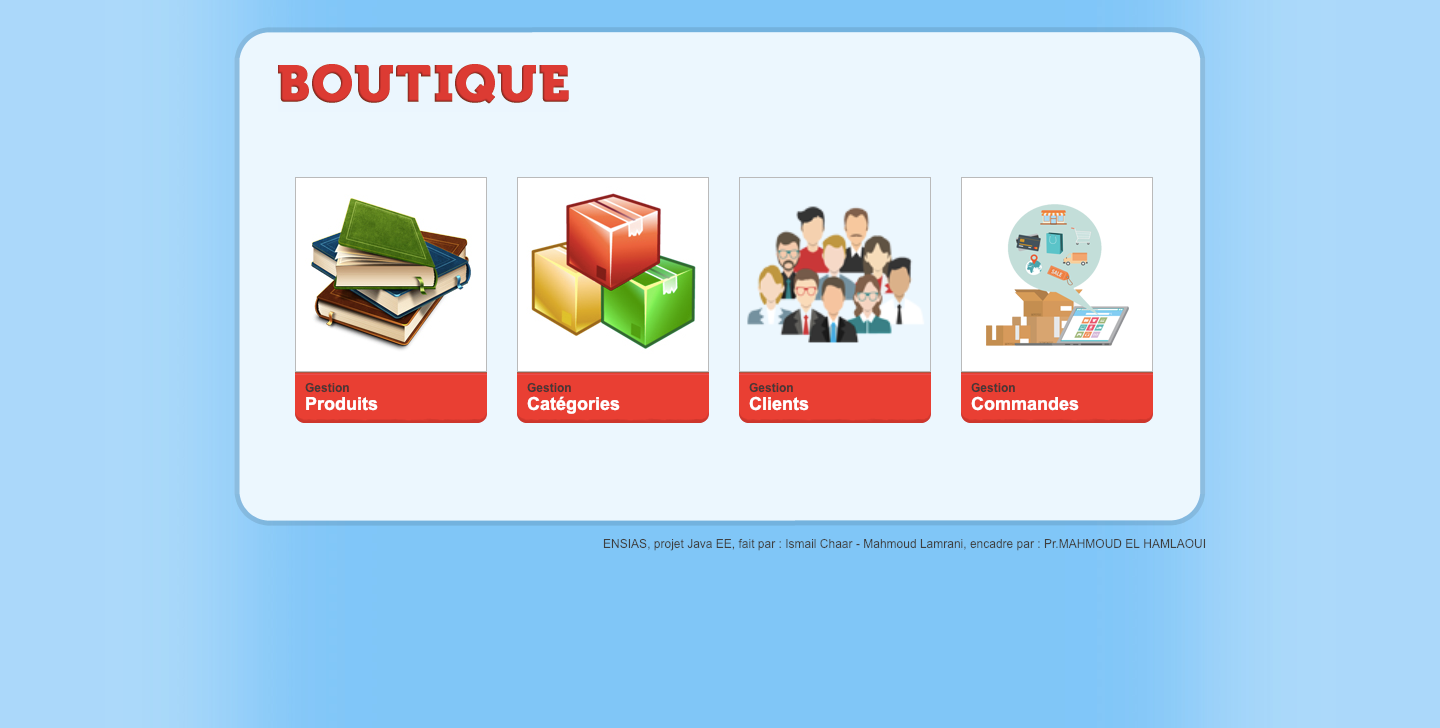
\includegraphics[width=\textwidth,scale=0.8]{screens/Home-Administration.png}}
    \caption{Capture d'écran de la page d'acceuil du BackOffice}
\end{figure}
L'application donne à l'administrateur la possibilité de gérer les livres, les catégories, les clients et les commandes.
\subsubsection{Gestion de livres}
Dans la partie gestion de livres, on a le suivant : 
l'affichage de la liste des livres existants dans l'e-boutique, avec toutes les informations : la première page de couverture, le titre, la catégorie, le prix et la quantité en stock.
La possibilité de supprimer, de modifier un livre ou d'ajouter un nouveau.
\begin{figure}[H]
    \centering
    \fbox{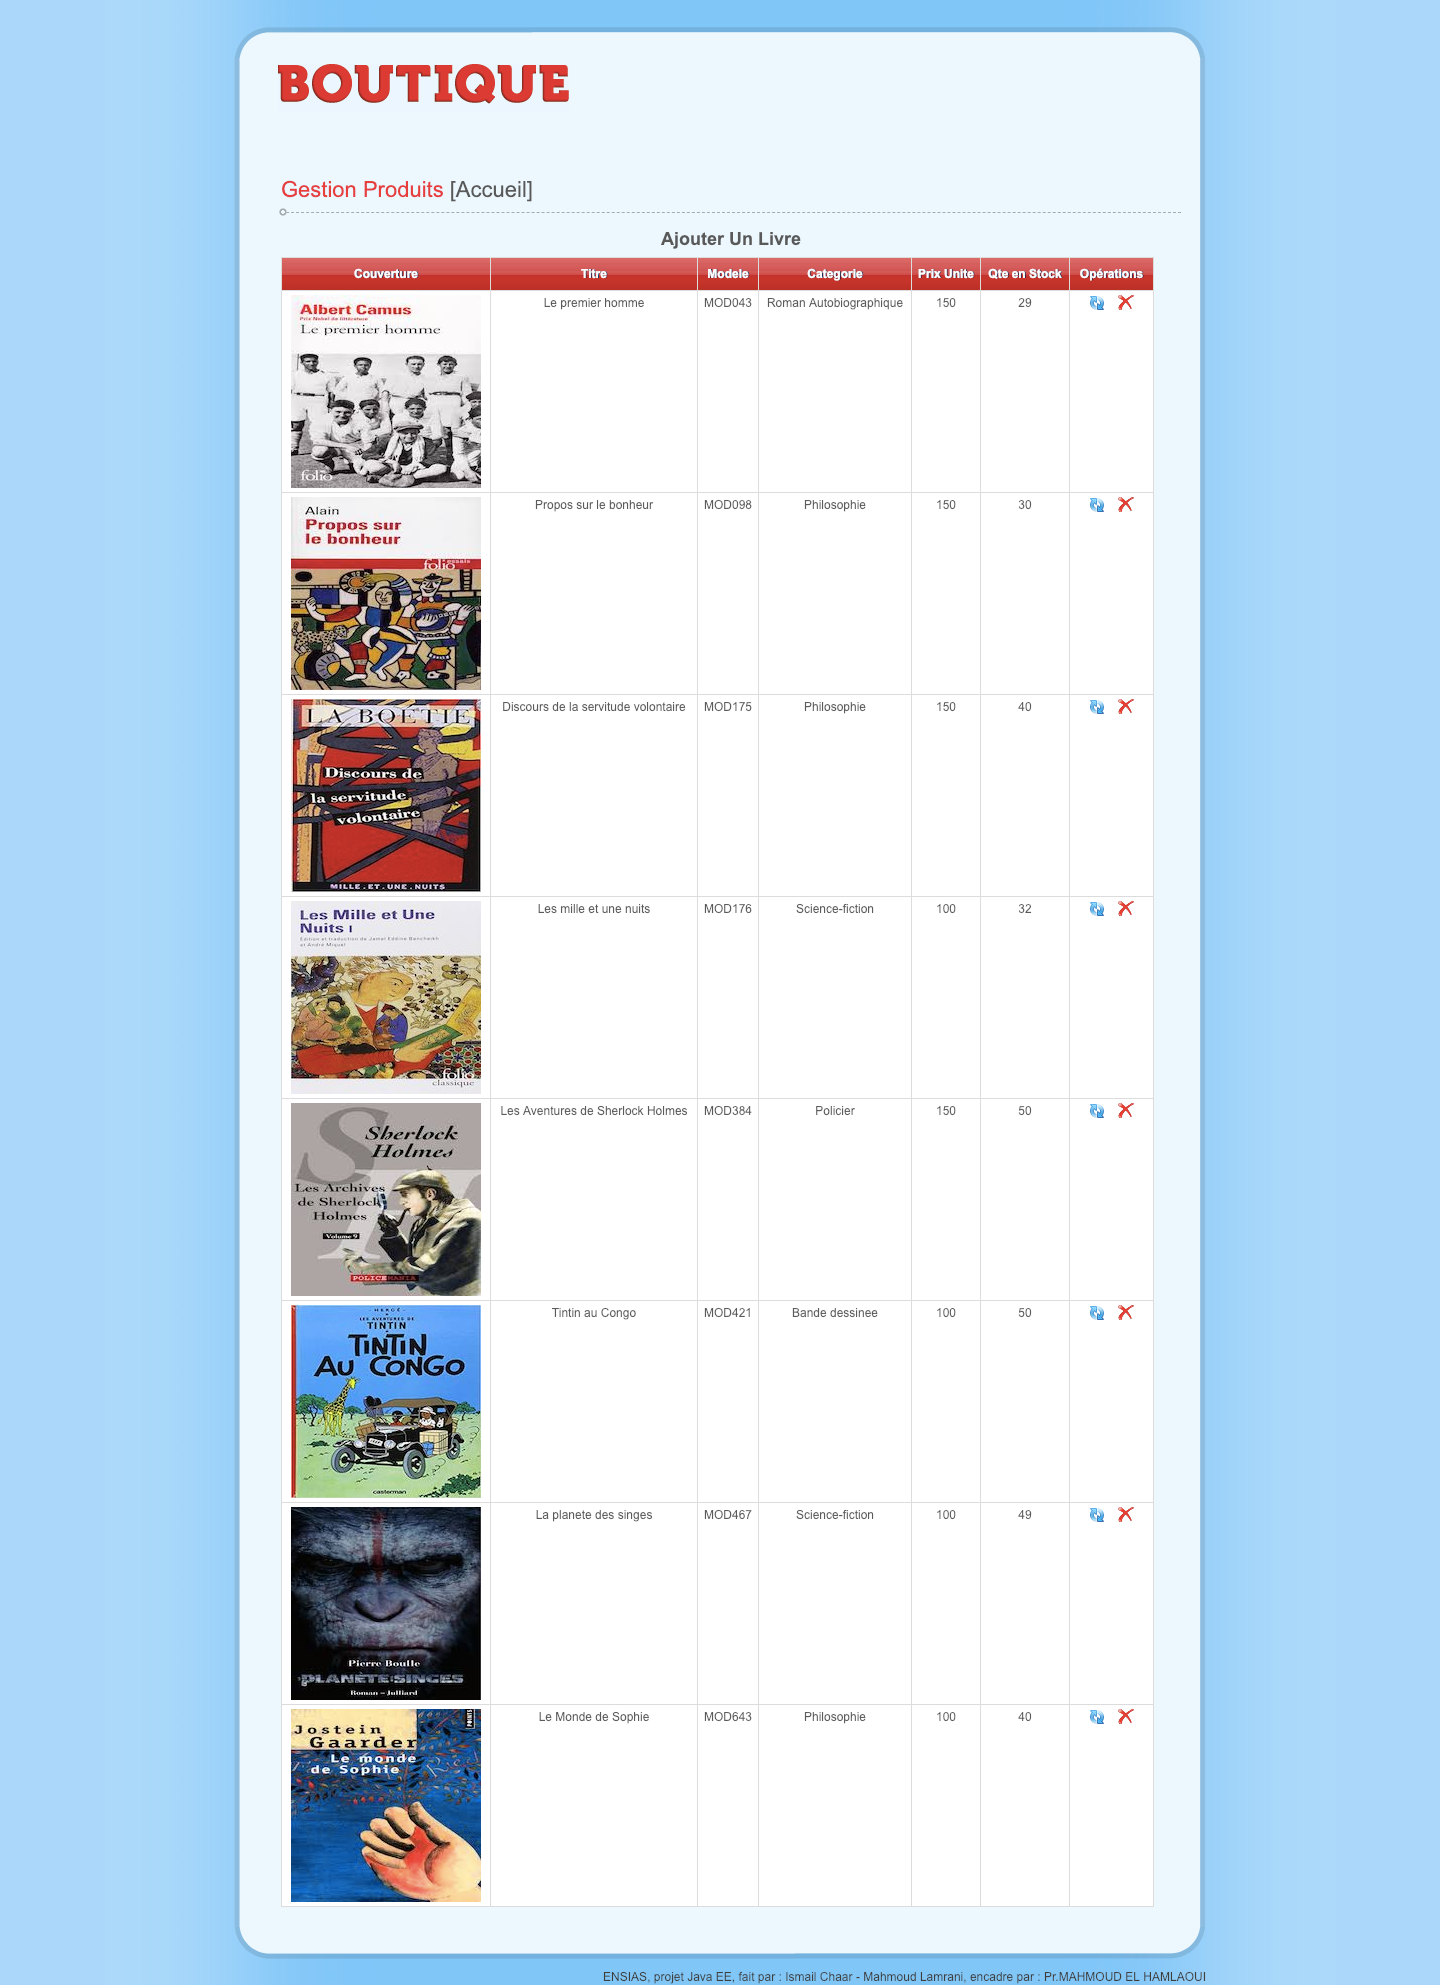
\includegraphics[width=\textwidth,scale=0.75]{screens/GestionProduits.png}}
    \caption{Capture d'écran de la page de gestion de livres}
\end{figure}
\begin{figure}[H]
    \centering
    \fbox{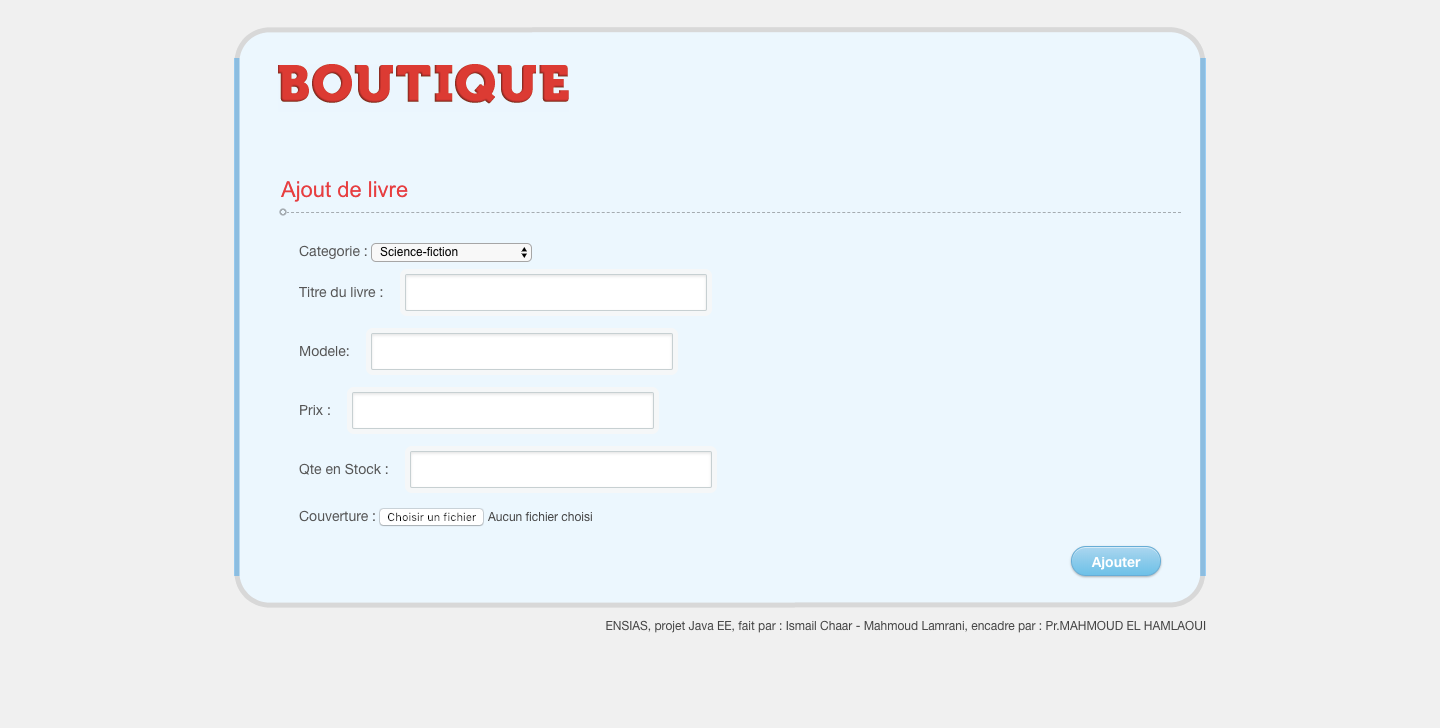
\includegraphics[width=\textwidth,scale=0.8]{screens/AjouterProduit.png}}
    \caption{Capture d'écran de la page d'ajout d'un livre}
\end{figure}
\subsubsection{Gestion de catégories}
Pour les catégories, on affiche toutes les catégories de livres dans le site, on peut soit supprimer une catégorie, modifier son libellé ou bien en ajouter une nouvelle.
\begin{figure}[H]
    \centering
    \fbox{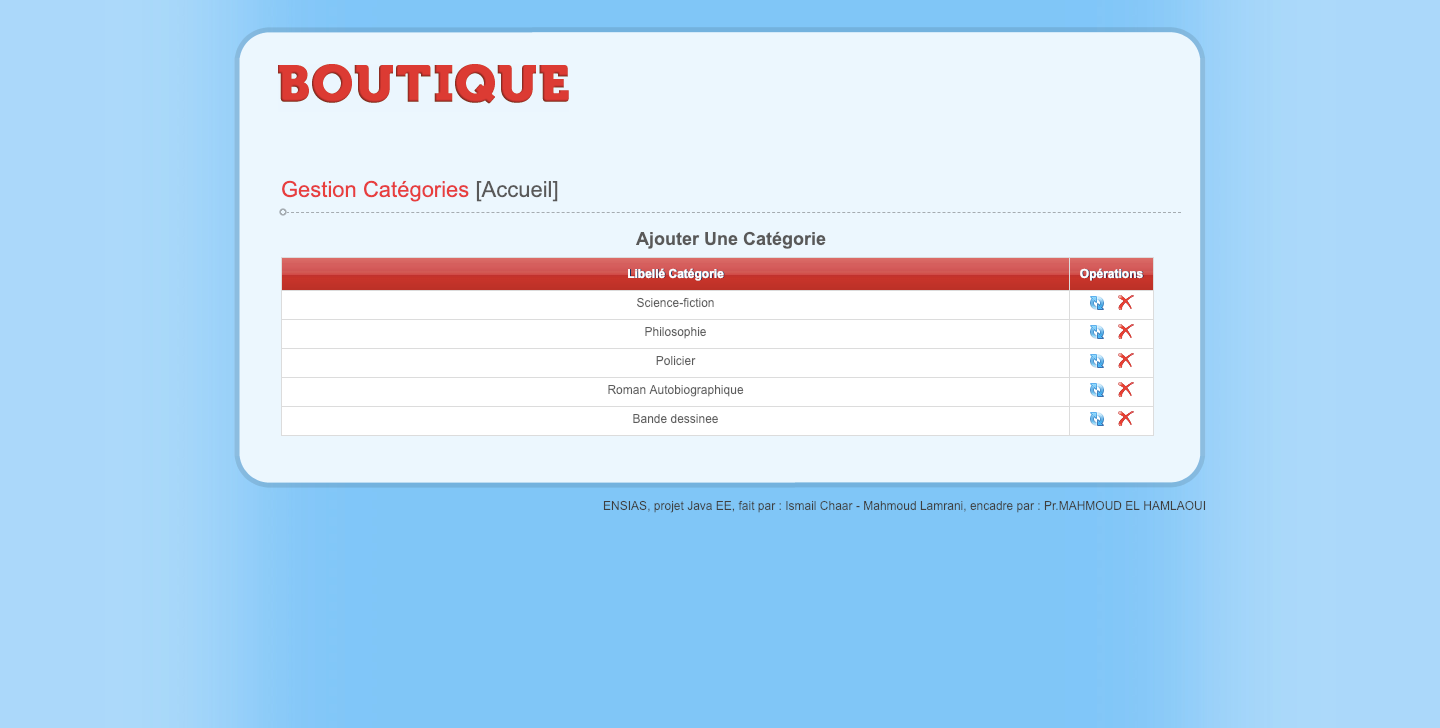
\includegraphics[width=\textwidth,scale=0.8]{screens/GestionCategories.png}}
    \caption{Capture d'écran de la page de gestion de catégories}
\end{figure}
\begin{figure}[H]
    \centering
    \fbox{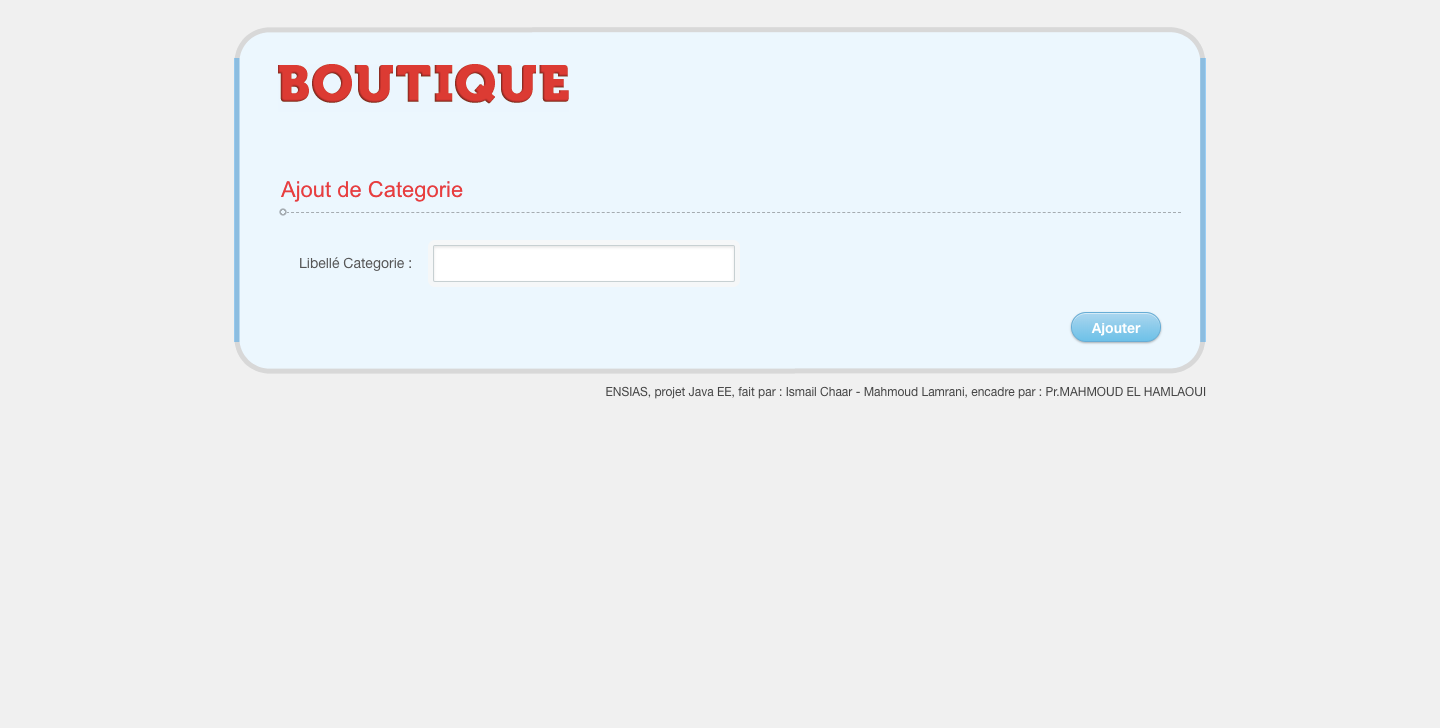
\includegraphics[width=\textwidth,scale=0.8]{screens/AjouterCategorie.png}}
    \caption{Capture d'écran de la page d'ajout d'une catégorie}
\end{figure}
\subsubsection{Gestion de clients}
Pour le volet consacré à la gestion des clients, on affiche les informations de tous les clients de l'e-boutique (nom, adresse, e-mail...) avec la possibilité de supprimer un client.
\begin{figure}[H]
    \centering
    \fbox{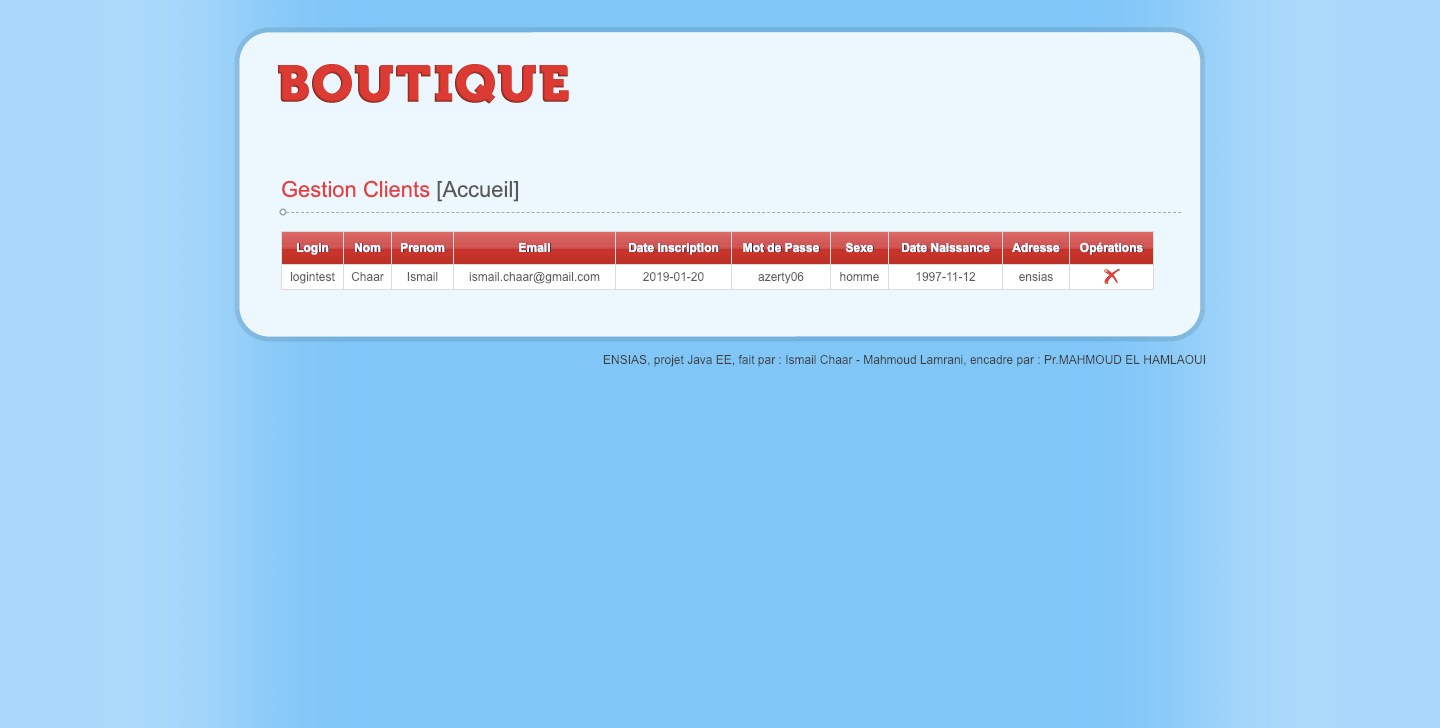
\includegraphics[width=\textwidth,scale=0.8]{screens/GestionClients.png}}
    \caption{Capture d'écran de la page de gestion des clients}
\end{figure}
\newpage
\subsubsection{Gestion de commandes}
On affiche toutes les commandes effectuées par les clients du site, leur prix total, ainsi la possibilité de valider ou non une commande.
\begin{figure}[H]
    \centering
    \fbox{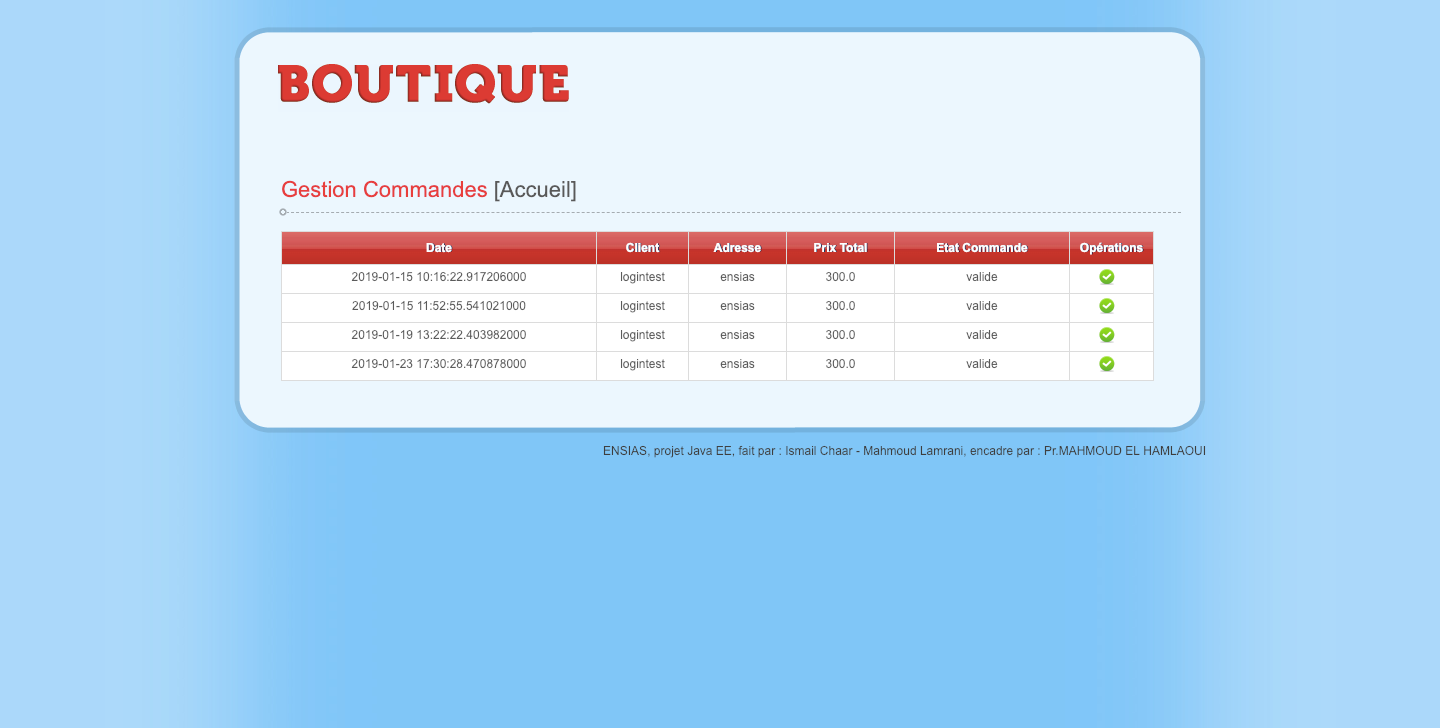
\includegraphics[width=\textwidth,scale=0.8]{screens/GestionCommandes.png}}
    \caption{Capture d'écran de la page de gestion des commandes}
\end{figure}
\subsection{Le FrontOffice}
Le front office est la partie d'un site internet qui est visible par les internautes, celle que l’on consulte et que l’on atteint par l’adresse internet (URL)
\subsubsection{L'acceuil}
Ceci est la partie d'accueil de notre site, on fait représenter un Slider descriptif de quelques livres, on affiche les différentes catégories des livres de l'e-boutique et on montre les nouveaux livres ajoutes à l'e-boutique sous la rubrique Nouvel Arrivage.
\begin{figure}[H]
    \centering
    \fbox{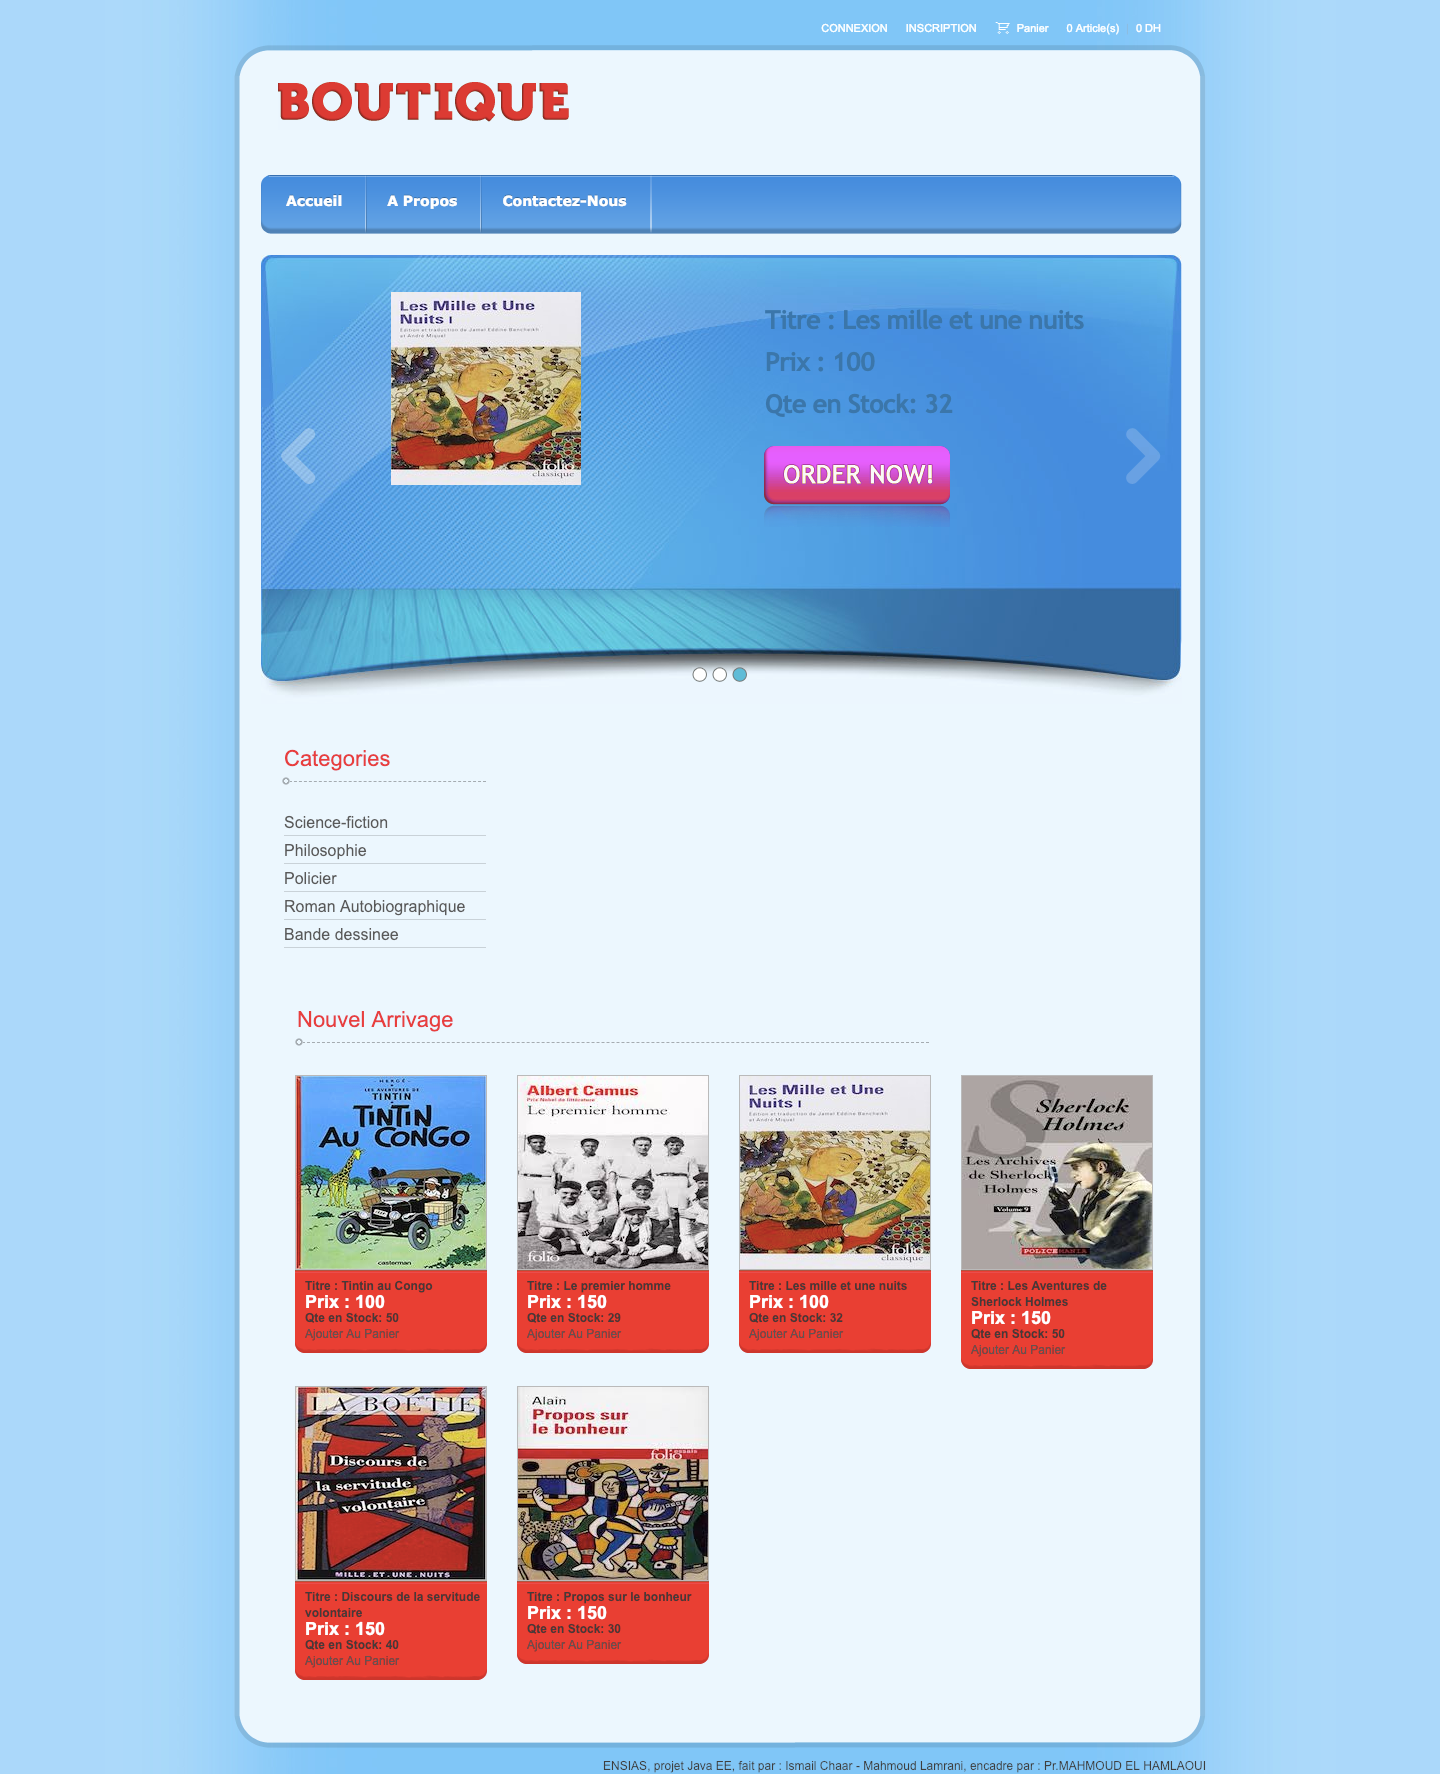
\includegraphics[width=\textwidth,scale=0.8]{screens/Home-Client.png}}
    \caption{Capture d'écran de la page d'acceuil du FrontOffice}
\end{figure}
\newpage
\subsubsection{Authentification}
Pour l'authentification, le client a la possibilité de se connecter s'il a déjà un compte via le formulaire de connexion ou bien de créer un nouveau compte en donnant quelques informations demandées via le formulaire d'inscription.
\begin{figure}[H]
    \centering
    \fbox{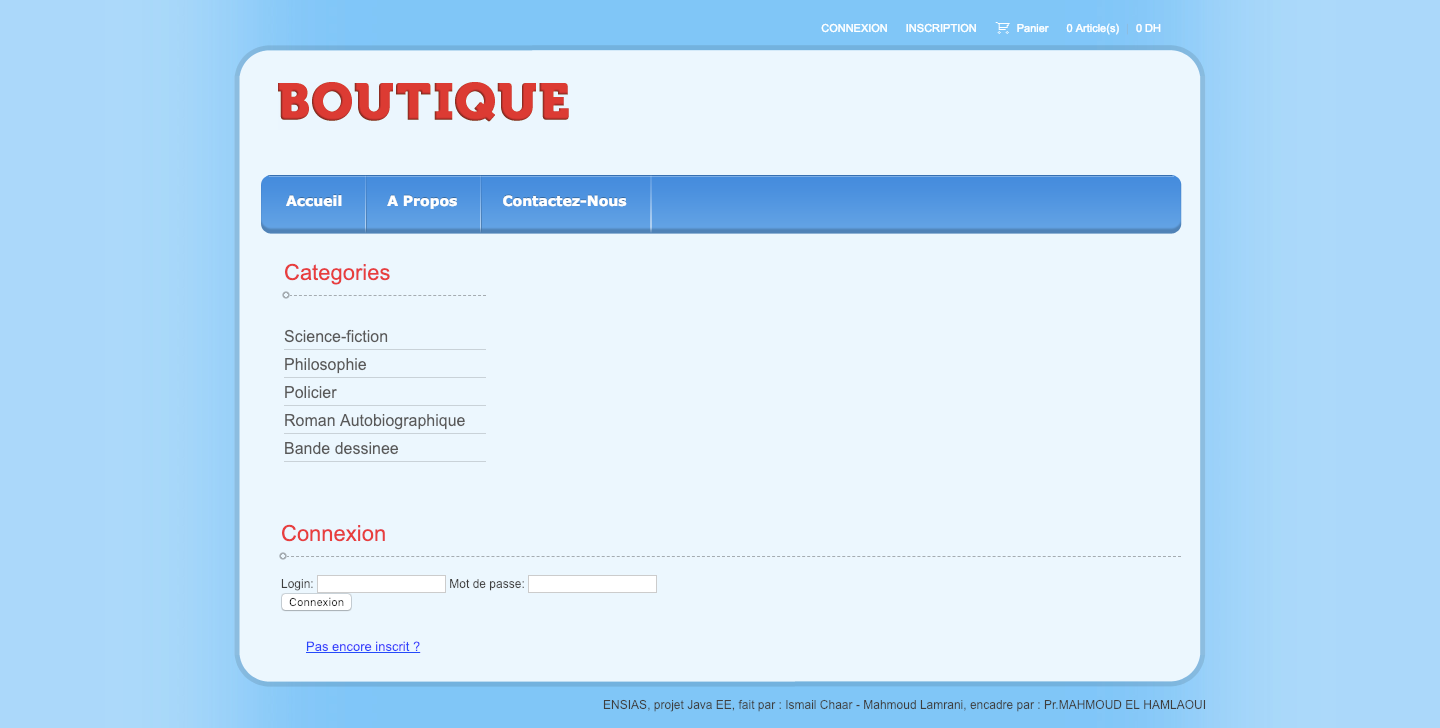
\includegraphics[width=\textwidth,scale=0.8]{screens/connexion.png}}
    \caption{Capture d'écran de la page de connexion}
\end{figure}
\begin{figure}[H]
    \centering
    \fbox{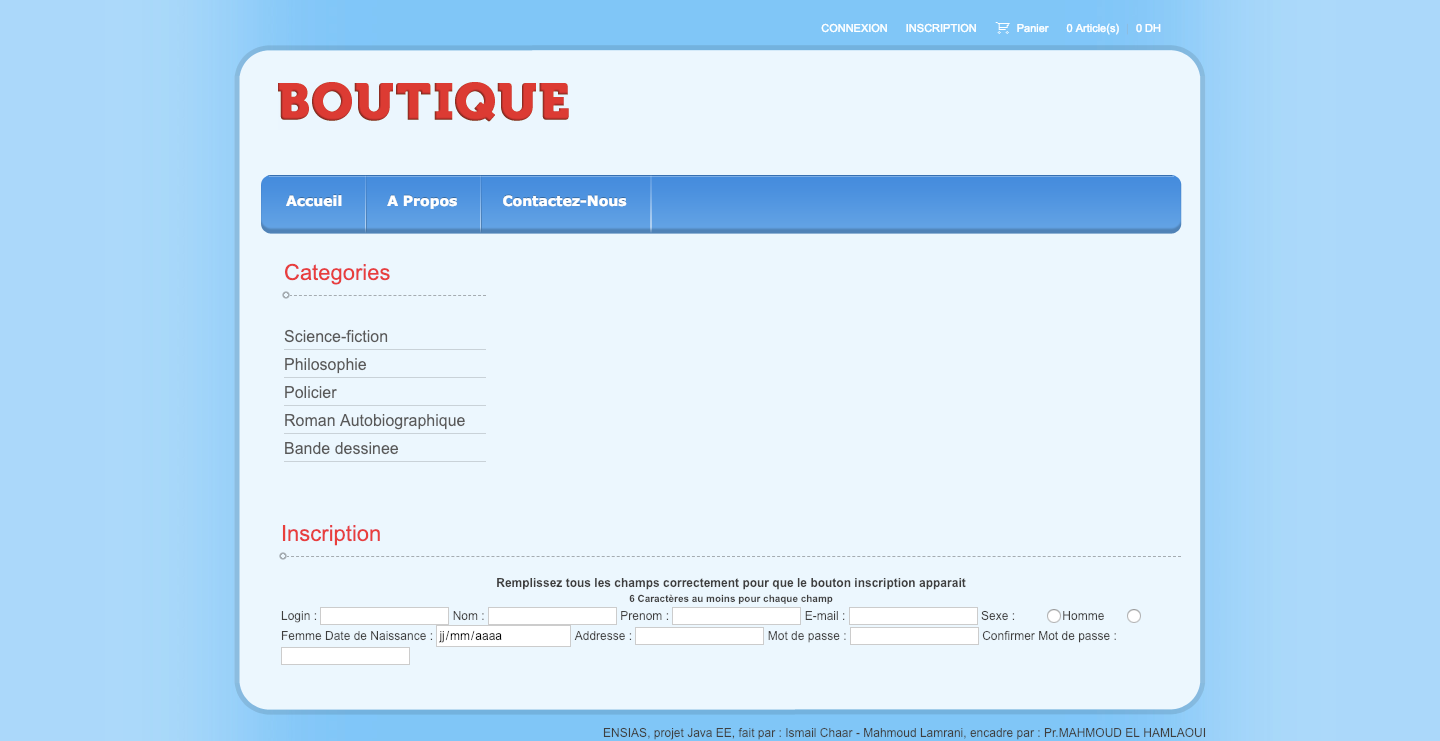
\includegraphics[width=\textwidth,scale=0.8]{screens/Inscription.png}}
    \caption{Capture d'écran de la page d'inscription}
\end{figure}
\newpage
\subsubsection{Panier}
Après avoir sélectionné un livre la page du panier s’ouvre, le client aura trois possibilités de soit cliquer sur « poursuivre les achats » pour choisir d’autres produits, soit cliquer sur « Passer la commande » pour effectuer son achat, soit cliquer sur « enregistrer le panier » pour avoir la possibilité de continuer son achat même après déconnexion.
\begin{figure}[H]
    \centering
    \fbox{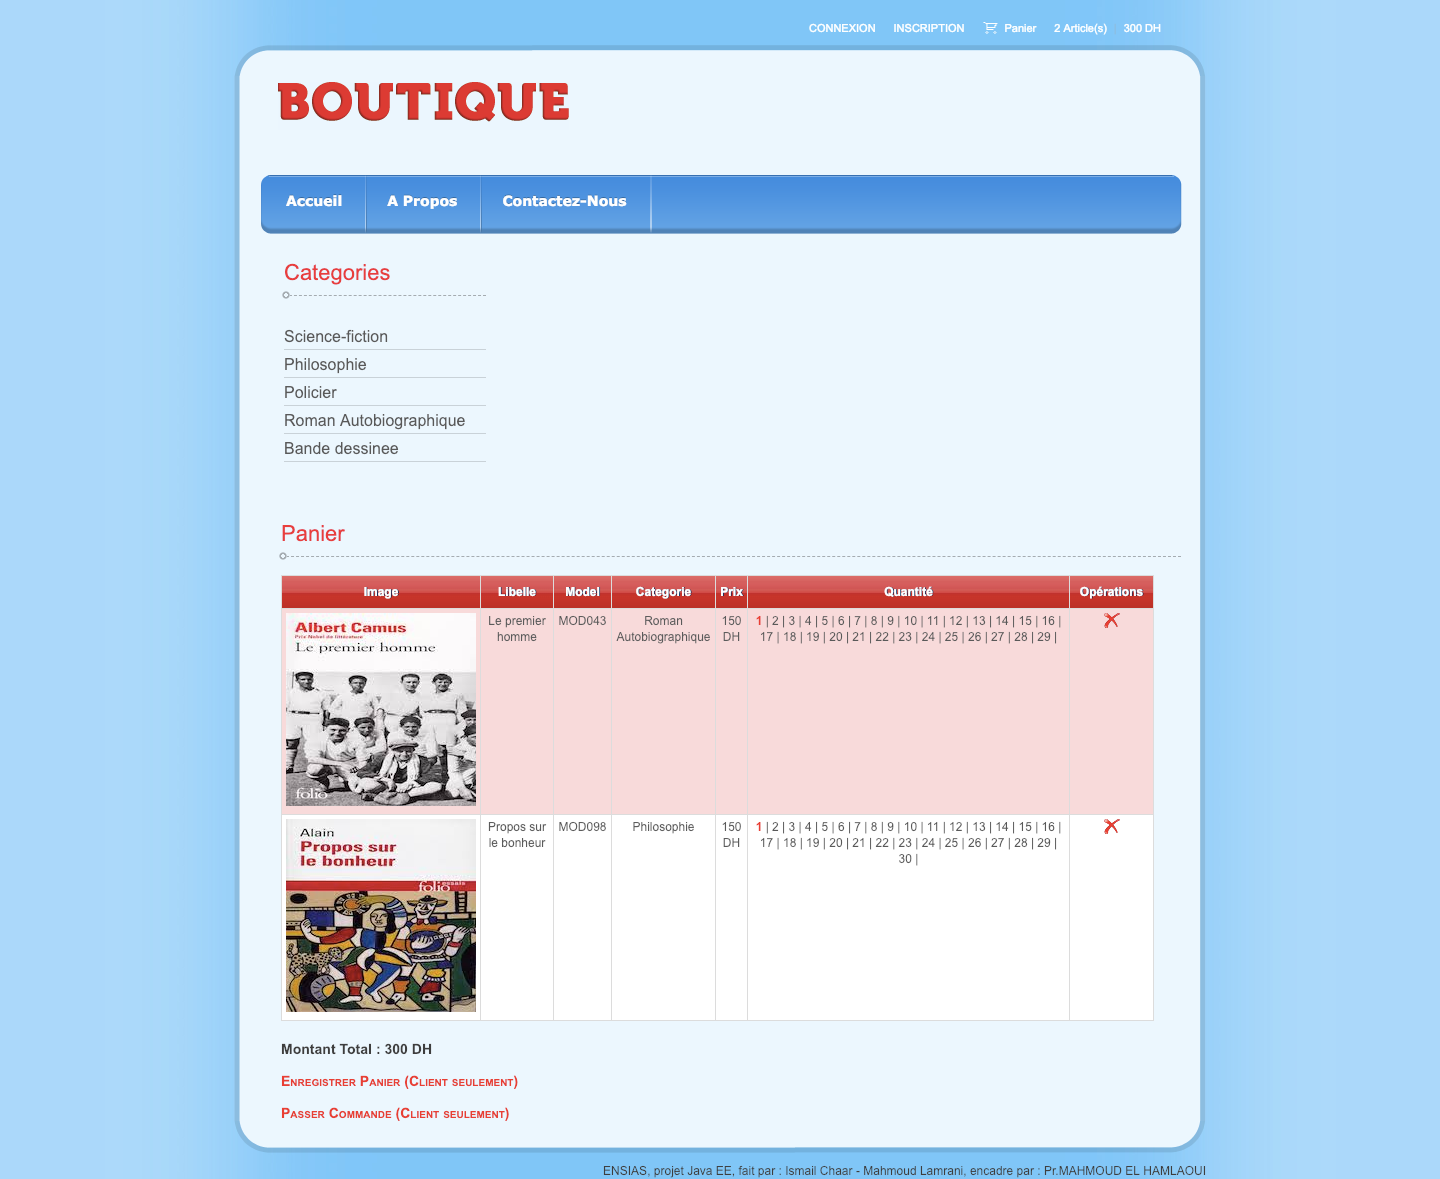
\includegraphics[width=\textwidth,scale=0.8]{screens/Panier.png}}
    \caption{Capture d'écran de la page du panier}
\end{figure}
\newpage
\subsubsection{Espace client}
L'espace client affiche au client ses propres informations, ses commandes et son panier enregistré.
\begin{figure}[H]
    \centering
    \fbox{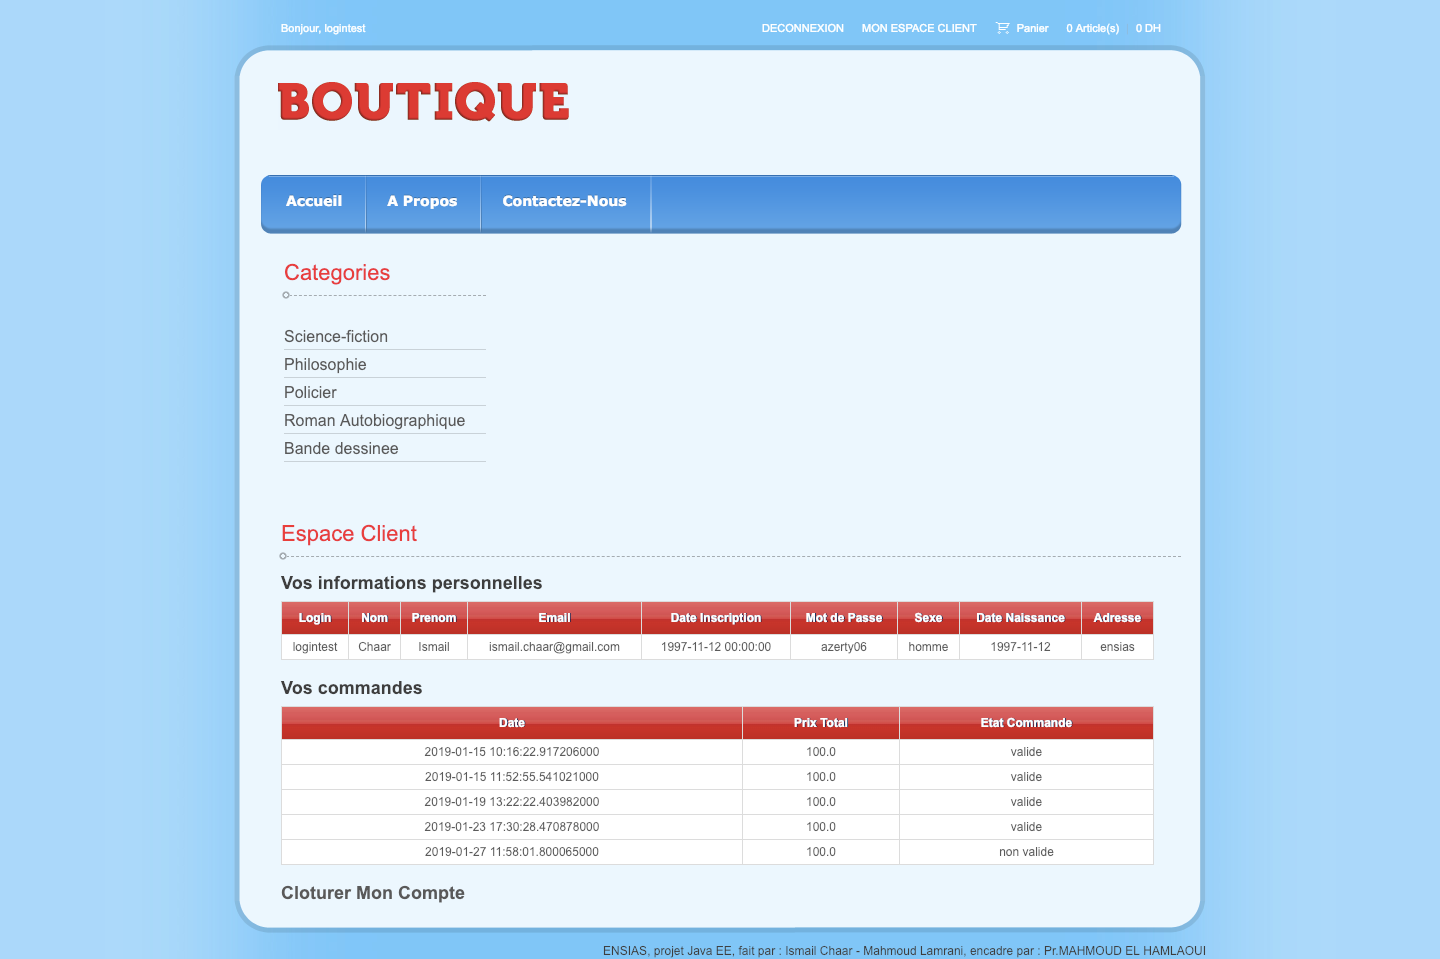
\includegraphics[width=\textwidth,scale=0.8]{screens/Espaceclient.png}}
    \caption{Capture d'écran de la page de l'espace client}
\end{figure}

